\documentclass[11pt]{article}
\usepackage{fullpage}
\usepackage{cite}
\usepackage{datetime}
\usepackage{geometry}
\usepackage{graphicx}
\geometry{verbose,lmargin=3cm,rmargin=3cm}

\title{Automated negotiation in the game of diplomacy - Final report}
\author{Matthias Hueser, Andras Slemmer, Luca Deltodesco, Luke Tomlin, Cliff Sun}
\date{\today}

\begin{document}
\maketitle

\begin{Abstract}


\end{Abstract}

\tableofcontents

\section{Acknowledgements}

\section{Introduction}
The Game of Diplomacy is a round-based multiplayer strategy-game set in post WWI
Europe. Each player controls a power which initially operates from a number of 
home-bases. The ultimate objective of each player is to control the majority of
supply-centers on the map. A game is structured into a number of rounds, in which
each player formulates a move order to conquer additional supply centres or
defend existing ones. Besides the necessity to create effective long-term
strategies negotiation is integral to the game-experience. There is a thriving
internet-based community around the Game of Diplomacy and many AI players, so
called bots, have been created in the past. Most of the existing AI players are
quite effective decision-makers in general but few of them support negotiation
or reasoning about the relationship of the powers in the game. Our project aims
to create a framework for Diplomacy, including a GUI client, a game server and a
collection of bots. Crucially the highest evolution of our series
of bots should be able to analyze and act upon messages of human / AI players and
issue messages to other players. Finally experiments are conducted to determine whether
there is a reward associated with negotation capabilities. This will require
careful study and implementation of automated negotiation techniques from other 
domains in AI/Game Theory. Thus the project gives us ample opportunity to be
creative and test different approaches using the DAIDE-conforming game framework
also produced for the project. DAIDE is a standard client-server protocol which
serves as a 'common language' for different Diplomacy bot implementations, 
enabling them to play a game together on a conforming server.

\section{Background and Related work}

\section{Requirements}
High-level requirements were discussed in the initial phase of the project 
(weeks 1/2) with our project supervisor -- Iain Philipps -- who is our customer
in Software Engineering terms. The terms of the collaboration were such that 
only certain high-level goals were defined and decisions about which AI techniques
to use were left with the team-members.

\begin{itemize}

\item The over-arching goal and hence the most critical requirement is to 
      design and implement a negotiation bot for Diplomacy whose performance
      is then compared to existing bots in an experimental setting. 
\item A collection of other bots which are not capable of commuication should
      be created for purposes of comparison. These should use proven techniques
      from the fields of Game Theory and Multi-Agent systems, including learning,
      tactics and long-term strategies. All bots should support the DAIDE 
      protocol to compete against existing bots on the DAIDE windows server.
\item To facilitate experimentation an open-source framework conforming to the
      existing DAIDE protocol should be created. This framework comprises a 
      server which hosts games for automated and human clients and a tool to
      gather game statistics. The imperative behind this is to feed-back
      into the Diplomacy community as a whole, providing a multi-platform
      server (Windows DAIDE server exists) for the first time. 
\item In addition a framework for simple generation of Diplomacy bots is 
      envisioned: Right now a player needs to re-invent the wheel by 
      implementing well-established game-tree search techniques or certain
      Machine Learning paradigms in low-level terms. This is clearly 
      unsatisfactory. Our framework helps to shift the focus to interesting
      new techniques from academia which can be coded up and layered on top
      of primitives. Actually this framework is used for the 2nd objective above
      to quickly generate a series of bots with increasing functionality.
      (Abstract client pattern) This also works as a proof-of-concept for the
      server framework. At the users convenience extensions are
      written in the high-level language Haskell which is more expressive than C++ 
      and natural to practitioners in the field of Artificial Intelligence / Game Theory.  
\item Finally to test our server and provide a visually pleasing user interface
      we will deliver a DAIDE-conforming GUI client for the Game of Diplomacy. 
      Rather than forcing the player to use a particular device all back-ends
      of the HaXe platform are supported, including HTML5/JS, Flash and C++. 

\end{itemize}

In the above listing the requirements are decreasing in importance. Some of
the above look indivisible in nature but we have still managed to
extract user-stories to support time-boxed iterations. Requirements management
in Weeks 3-11 was two-fold: Each team-member kept in mind the overall contract
with our supervisor (see above) which defines the direction of the project. 
Based on this User-Stories were defined which guide the primary development
focus during the iterations.

\subsection{Change management / Risk mitigation}
We recognized that change is inevitable in such an ambitious and multi-faceted
project. Therefore we took great care in defining our contracts carefully to
split up work. Actually this was helped substantially by the existence of the
DAIDE protocol. Through its rigorous specification it forced everybody to 
program to an existing interface and there was little scope for confusion as
to what needs to be supported. 
\\
Each of the high-level objectives outlined above can be achieved
separately and as a result there are little dependencies between team members.
If communication between two components fails it is matter of determining
which are not properly realizing the DAIDE protocol. A welcome side-effect
is that we avoid endless debugging sessions to make two parts of the project
work together. They just need to be tested against a DAIDE reference.
\\
Using the 'AI generation' framework explained above implicitly makes coding 
of AI techniques incremental. For instance if a well-tested game-tree search
or Learning algorithm is in place, each evolutionary bot can delegate
these tasks without worrying about how they are implemented. Turning this
into a reality required defining a layered design in Weeks 3-5 which all
future work respected.
\\ 

\subsection{Planning / task estimation}
All planning took place in the weekly group meetings (for the structure
of a meeting see example at the bottom of document ). A general rule for
new user-stories was that they relate to the global objectives defined
in the contract with our supervisor (see above). This avoided falling ill
with 'featuritis' at any point in the project. 
\\
In the AI realm a new user story was typically introduced
by a team member. Generally we shied away from implementing exotic
algorithms that are not clearly understood by all team members, adopting
the ``Kiss principle''. Also there should be a balance between different
paradigms in the AI design, which enables us to make meaningful 
experiments for the final report. For instance it is not seen as fruitful
to performance-tune beyond the point where much value is generated on the
whole. Rather the focus should be on negotation. Associated with each
user story we started a quick poker game to estimate the required
time-resources for completing the feature. Obviously members with more
experience in a domain were given more weight in the decision process.
We usually arrived at a decision about a future iteration unanimously.
\\ 
For the server the process was less creative and controlled by the
need to conform to the DAIDE protocol. Conversely planning was 
easier because the process of creating a parser is understood by 
all team members.

\subsection{Progress metrics}
There are multiple ways in which we can measure the progress of our AI. 
We adopted an aspect-oriented approach in measuring, recognizing that 
some requirements are fulfilled qualitatively and others can be stated
in terms of numbers.

\begin{itemize}
\item A natural but informal progress metric is to simply estimate for
      each high-level objective defined in the contract a percentage of the
      features which have been successfully implemented. This places emphasis
      on the big picture rather than measuring the performance of a particular
      bot we have created.
\item Another metric which only pertains to the AI side-of-things is a
      quantative measure of how do we fare against typical existing bots. Such a
      metric could be gathered for example in a Round-Robin tournament. 
      As a canonical example we adopted the existing DumbBot which despite its
      name has considerable playing stregth. According to our supervisor
      systematically out-performing DumbBot presents the technical benchmark 
      for the project.
\item Relevant to the server-framework and the GUI client we can define a 
      measure by the percentage of valid DAIDE messages supported. Once this
      is close to 100 \% it immediately follows that both are DAIDE-conforming,
      one of our objectives outlined above.
\item As a GUI is hard to test automatically we left 10 mins of our weekly 
      discussions for informal game walkthroughs. All team members judged how
      natural / visually pleasing the interface was and what features could
      be supported in the next generation. We have not used any formal methods
      here but trusted our experience with playing similar strategy games.
\end{itemize}

\subsection{Detailed AI metrics}

Within each of these milestones, we can weigh a bot's ability using its only 
application - playing the game of diplomacy. For this, we need to come up with
a set of metrics with which we can evaluate a players performance in a game. We
are planning to equip the server with a tool to measure these statistics during
the game. By combining these indicators in a weighted fashion (possibly with
some needed calibration), we should be able to compute an accurate score of how
well a particular AI is playing. This can be validated by measuring the
correlation with a high-score and the number of games won/lost.
\\
Some key indicators are, with some having precedence over others:

\subsubsection{Games won/lost} 
This is clearly the most important metric and overrides all others.
However it gives little insight into what actually caused a bot
to lose or win the game.

\subsubsection{Supply centres controlled}
With regards to supply depots, the winning player will own half of them 
(eighteen), with the second-most successful player owning the second highest 
amount, and so on and so forth. A player with no supply-depots is very close
to becoming a losing player.

\subsubsection{Units lost during the game}
Units lost is a difficult metric to quantise - whilst it may immediately seem
that losing many units is a bad thing, these could be due to tactical masteries
involving trappingand deluding many foes. Objectively, it is probably advisable
to refrain from losing units where possible.

\subsubsection{Provinces conceded during the game}
Similarly, conceding provinces, unless done in a planned fashion, is a general
indicator that a player is not performing well.

\subsubsection{Negotiation 'strength'}
If it were possible to evaluate other players' "attitudes" towards
the AI player, one might be able to deduce the competence of a bots negotiating
skills. For instance, making enemies is widely regarded as a poor move,
especially if those enemies are actively hostile against you. A better tactic 
might be to give them the illusion of friendship, whilst aligning them for a
back-stabbing manouever. If we could create a way to reliably score the 
subtleties of negotiation between players, it might aid us in the creation of
more advanced diplomising AIs.

\subsection{Team velocity / Milestones}
We can define our team velocity as the positive change in progress metrics overall. 
This means that we can allocate team members to the metric which currently has 
priority. These are typically the ones that are covered by the user-stories for
the current iteration. Having said that we strived to progress in each part
of the project to discover problems and dependencies we have not anticipated
early. 
\\
Whereas the velocity-scheme served as a tool to measure our progress internally
we communicated our progress to the supervisor in terms of coarse-grained 
milestones. This had the advantage that we did not overload our customer with
technical details that only we as developers care about. Also they co-incided with
the frequency of meetings with our supervisor. 
\\
The milestones agreed upon were to create the AI framework and the server, and then
proceed to iterate a build of an AI, progressively increasing its abilities and
making it better. 

\subsection{Description of iterations per subsystem}

\subsubsection{Framework and Server}

For the server we can define some functionality 'chunks' which are strictly 
independent from others, these guided how we allocated user stories to the
3 iterations outlined below:

\begin{itemize}
\item First and foremost the server needs to conform to the DAIDE specification which
      is an issue of setting up a connection between server and client and parsing
      conforming issues. This is a well understood task from the 2nd years Compilers
      course and hence it formed our first iteration. At the end of the iteration
      substantial testing was performed (see section on Testing for details). Notice
      there is no dependancy on any other component being working.
\item Secondly the server needs to advance the game state in response to valid
      DAIDE messages. This was a longer iteration since all special cases 
      treated in the game rules needed to be catered for. Again existing bots and
      GUI clients could be used to instrument the server and validate correct
      reaction.
\item The last iteration of the server consisted of User-Stories which were 
      created during the weekly meetings. They were not strictly necessary but
      but useful utility features that served to round up the product. Free time
      was now spent on refactoring the code and fixing remaining bugs.
\end{itemize}

\subsubsection{AI framework / bots}

These iterations have run concurrently with server developments (3 iterations
detailed above):

The user stories we have proposed largely correspond to ideas DAIDE wiki and
research into machine learning / search techniques. 
\\
Each user story contains an iteratively improved version of our current 
benchmark bot. Hence the overall AI gains functionality and depth on each
iteration. While there are some components which every bot should have (for
instance a forward-search in the game state-space) specifics are discussed 
during the group meetings. The idea is that each team member involved in 
the AI has done some research and proposes new AI techniques which shall be
implemeted in the next time-box.
\\
Then once a feature is judged mature we incorporate it into the generic AI
framework discussed at the beginning. This extends the code-base we treat as 
given for the next iteration. 

\begin{itemize}
\item The first iteration -- HoldBot -- is simply an AI player that does not
      impede the game progress. It always performs the same move -- it holds.
      It can be used as a simple unit test for the server framework.
\item As a first refinement is RandomBot is created, which now considers every
      move defined in the Diplomacy rules and selects one uniformly at random. 
      Reflection capability is optional, that is the bot may or not reason about
      how the random moves affected its standing in the game.
\item The first bot designed to compete with other bots through the DAIDE protocol
      is StrategyBot. At a high-level it must use techniques for performing
      a search in the game tree, formulate general strategies. Also it should be 
      able to improve its performance by analyzing previous strategies or moves.
\item The last iteration is the NegotiatingBot which additionally exchanges 
      messages with other players. It needs to have an internal model of the other
      players intentions and reason about which is friend or foe.
\end{itemize}

\subsection{Progress report for Week 10/11}
Unfortunately we suffered some setbacks in the beginning with planning and 
evaluation of how long it would actually take us to complete the server and
framework. These miscalculations have now been addressed and we are progressing
with the AI creation while improving server / framework as appropriate. 
\\
On the AI-side HoldBot and RandomBot are released (to the current specification of the
AI framework). The current iteration focusses on implementing the features of
StrategyBot.


\section{Software architecture}

\subsection{AI methods}

\subsection{Negotation methods}

\section{Validation}

\subsection{Server testing}

\begin{itemize}
\item A very practical and simple method for us to test the server is to let
      RandomBots join a game and issue arbitrary move commands. We estimate that
      we get good coverage using this method since a random bot is expected to
      issue every possible move over a large number of games. We expect that
      the server does not crash and advances the game state correctly. We check
      successful completion by checking for any error return codes / exceptions
      thrown by the server. The latter is tested by cross-checking the game state
      with the Windows DAIDE server which we forward all messages that our server
      receives. Since both observe the same game the messages send to clients 
      should not differ. To automate the tests, we created a script that 
      intercepts client-server communication and then invokes 'diff' on the
      messages. 

\item To inspire further confidence in the code's correctness we use the Quick
      Check tool developed for the Haskell platform: Given pure Haskell code
      (that is containing no I/O) it generates random function inputs
      and theoretically allows us to test a function exhaustively. For instance
      to test a parsing function we can specify the invariant that it accepts
      precisely the members of the DAIDE language and returns a parsing
      error otherwise. For the 'state advancing logic' of the server we can
      check certain properties that we know to be true in general. An example
      would be: A supply centre can only be conquered if an army of the
      player was sent there. We decided against a parallel module hierarchy for
      the tests but instead defined submodules of the form 'X\_quickcheck'. 
      This allowed us to use the tests as documentation when writing the
      functions and avoided synchronization issues. This also facilitates 
      testing of functions that are not exported from a module. 

\item To augment testing with QuickCheck one team member has encoded a number
      of representative game situations as unit test cases. Largely these
      were taken from the DiplomacyRuleBook, one of the references
      that specifies correct state advancement. The unit tests 
      were written in HUnit, whose feature-set largely parallels JUnit for 
      Java programming. The whole testing framework can be automated, tests 
      being packages hierarchically in test suite, modules and collections.
      As QuickCheck tests they live in a module sub-
      ordinate to the functions tested. 
\end{itemize}

\subsection{AI client testing} 

\begin{itemize}

\item A very simple test is to determine whether an AI client does not
      impede the progress of the game. This can simply be tested by letting 
      the client on either the functional Haskell or the existing DAIDE
      server (Windows). The script running the test will intercept any 
      error messages issued to the client and deem the test to be failed
      if any syntax errors (no valid DAIDE message) or semantic errors
      (moves that do not make sense with respect to the current game-state)
      were flagged.

\item Anything that goes beyond liveness and absence of errors cannot be 
      tested trivially. Instead of testing we let bots play in Round-Robin
      tournaments, collect game statistics and assign each bot a playing
      strength metric. The exact way and the ingredients of the formula
      were outlined in the section on 'AI metrics'. Ultimately playing
      strength equates to faring robustly against a large collection of 
      existing bots.

\item Some white-box testing was done to determine how the AI arrives at 
      a decision and check if its reasoning is sound. We designed the different 
      parts of our AI with testability in mind, often using very tiny
      functions. As an example consider an interface that measures the 
      utility of a game state to a certain player. It can be tested by 
      simply comparing the result with our pen-and-paper calculations. 
      Some of these tests were coded up as HUnit test suites. 

\end{itemize}

\subsection{GUI client testing}

\begin{itemize}

\item For the GUI client similar criteria to the AI client applied. The
      client should be live during the game and not issue mal-formed
      messages. A simple script that instruments the GUIs command-line
      interface was put in place for this.

\item Unit testing in the HaXe proceeded as recommended in its manual:
      Simple test cases to check correct parsing of SVG files (encode
      the map topology) were created by subclassing a TestCase and
      putting appropriate checks in place.  

\item Functional requirements were largely in-tangible, such as presenting a
      intuitive, visually appealing interface to the user. Our division of
      labour allowed that team members involved in the AI could give feedback.
      Roughly 15 mins of each meeting were dedicated to discuss the user
      interface: flagging new issues and tracking progress on fixing 
      previously discovered bugs. These tests were conducted for each
      end-user device targeted by the HaXe framework, such as mobile 
      phones or internet browsers.

\item While there exist tools for automated-checking of web interfaces 
      the team dismissed this as misguided effort better spent elsewhere.
      The marginal utility would be to know that all buttons worked correctly
      which can also be tested by manual inspection. 

\end{itemize}

\subsection{Examples of bugs discovered during testing}
\begin{itemize}
\item Grave errors when parsing certain DAIDE messages. This had to do with
      the ambiguity of the DAIDE grammar and a work-around needed to be found
      (discovered through QuickCheck testing)
\item Inconsistences on the server-side. This proved a pain to rectify and 
      to avoid such problems in the future we decided to come up with a 
      robust scheme for concurrency in the server code. (discovered through
      sporadic server stress testing)
\end{itemize}

\subsection{Static code checking / tools}
All deliverables, including code and documentation was produced using Emacs /
Gedit or other similar simple text editors. We have not used an IDE but several
Emacs modes and extensions (directory browsing) helped us to keep track of the
overall structure of the codebase. Our strategy to achieve good coding style
was readability was two-fold: Rather than making up our own coding standard
we have adopted the programming guidelines from ``http://www.haskell.org/haskellwiki/Programming.guidelines''. Secondly
each team member was required to run each (compiling) commit through 'HLint'
and the 'Haskell Style Scanner' and resolve issues if necessary. 

\subsection{Code documentation}

We treated documentation as a deliverable only second in priority to working
code. The coding standards defined at the beginning of the project detailed 
the style of documentation and good practices to avoid running-out-of-sync
issues.

\subsubsection{Developer documention}

Developer documentation consisted of JavaDoc-style comments for each data type,
typeclass (interface) and function documentation. The particular tool used
is ``Haddock'' which allows generation of API reference pages (HTML).

\subsubsection{User documention}
Besides documenting exported API through ``Haddock'' (primarily the AI framework
for creating Diplomacy Bots) we agreed that tutorials need to be written to 
explain typical use-cases of the library. Only then can we hope that our
library is re-used by other members of the Diplomacy community which was an
objective defined at the outset of the project. Team members agreed that once
we go public with our project (BSD open-source licensed) we also need to have
a Sourceforge website. 

\subsection{Code inspection / Refactoring}
Each function of the code is ideally represented in three different ways: as 
executable code, unit test and exported ``Haddock'' comments. For some trivial
cases one of the latter might be missing. This approach has simplified code
inspection and walkthroughs tremendously. In a typical 'design-check' session
which is conducted roughly fort-nightly a team-member will check a 
particular code in detail. This involves clarifying comments, naming of 
functions and checking overall soundness of design. Often major
refactorings were suggested as it was discovered that pieces of code were
conceptually similar and hence could be extracted into a common module. Not
only were we challenging our tendency to 'repeat ourselves' in the code
but also could spread knowledge about the code-base in the entire team. By the
regularity of refactoring / design effort we wanted to avoid that the code-base
grows out-of-shape and acquires ``technical debt''.

\subsection{Acceptance tests}
Acceptance testing has not yet been finalized. In a recent meeting 
with our supervisor we conducted a short walkthrough of the GUI to gather
feedback. The functionally we have implemented was received well, with some
minor changes suggested. Final integration / system testing will be done 
during the holidays and the first week of the Spring term. We aim to keep
our supervisor involved by sending regular screenshots of the GUI and 
results from the Bot-tournaments.

\subsection{Stress testing}

\subsubsection{Server loading}

Our server can be stressed by increasing its load, flooding it with malformed
messages in spirit of Denial-of-Service attacks. The overall aim is 
to find a threshold load under which our server just crashes. Another test is
to connect multiple AI clients that issue conforming DAIDE messages at a rapid
pace. The question then is whether the server still advances the game state
correctly. If this is not the case we would need to check the server code for
possible race conditions explicitly. Initial measurements indicate sufficient
robustness. 

\subsubsection{AI / GUI client loading}

In a similar fashion GUI and AI client can be run against servers issuing 
malicious messages at a rapid pace. We allow arbitrary behaviour in this
case, but the client should still discover the problem and disconnect 
safely. Similarly we have to defend against an adversary who addresses spam
to force our player to time-out during move generation.   

\section{Project evaluation / experiments}

\begin{comment}

\end{comment}


\section{Managerial Documentation}

\subsection{Collaboration tools}
We discovered that the best tool was actually gathering in front of a
white-board (we did not yet have IdeaPaint TM), sticking some user story
cards and talking through the overall design. Simplified UML diagrams and
examples were used to elaborate design alternatives at our disposal. Anything
that was of permanent value to the team was usually recorded in a logbook
(see example of a LogBook page below). For this purpose we assigned a member
to take minutes of each meeting and create a digest that would be put into
the issue-tracking system of GitHub. Other resources of GitHub, such as
progress, issue flagging and milestone setting were used sporadically. Next 
time we would probably use a more sophisticated tool for resource management,
enabling us to categorize research papers, coding standards, progress 
reports in a better way.

\subsection{Terms of collaboration}

\subsubsection{Working hours / patterns}
As suggested in the spec each group member spent the rough equivalent
of one working day per week on the project. We assured there is a
good mix of work to be done by each member, so that nobody will become
bored or disinterested by tedious work. Of course some long coding sessions
were needed to fix bugs and integrate components. We tried to work against
such problems though by having regular meetings where the design and
any bugs are discussed. 

\subsubsection{Group meeting conditions}
Each group meeting was held in the conference room opposite the labs. We
ensured that each member was free for the day afterwards to cater for the
fact that meetings sometimes had to overrun the expected time. Whiteboards
were used to discuss the design with UML / package diagrams.

\subsubsection{Group meeting structure}
Besides discussing user-stories and mini-milestones for the next
iteration group meetings were used to do the following things

\begin{itemize}
\item Assessing risks early: For instance we dedicated one half-session to 
      come up with a technique to cope with race conditions occuring on shared
      data structures in the server. Two team members had alternative solutions
      to this solution with the group finally agreeing with using Software
      Transactional Memory, which is natively supported in the Haskell GHC
      extensions. Another technical risk was using the DAIDE system, which is 
      legacy in nature (ambiguities in the grammar of DAIDE messages etc..). The
      team had to discuss how to proceed in these cases.
\item Defining testing strategies: As shown in the testing section we have used
      different techniques in some are more appropriate in certain cases. Usually
      the team member working on the code made a suggestion and argued their case.
      We reckoned that everybody had a stake in the decision because the code was 
      usually tested / reviewed by a person different from the coder. Issues of
      code coverage and general confidence into the code / testing suite were 
      also raised here. The overall aim was to make out weak spots that need
      urgent clean-up and improvement.
\item At the beginning of each iteration, we plan out the work distribution that needs
      to be done. If more than one person is writing code we need to raise awareness 
      of dependencies that we may have between these members. These could take the
      form of overlapping code or module dependencies. Before any coding starts
      the respective members need to agree on a common strategy to avoid code duplication
      and factoring common parts out.
\item Each second meeting we try to do some ``meta-learning'' - that is what went wrong
      and how can we improve our process in the following week. For instance it was 
      discovered early that different knowledge bases about Haskell / monads could
      prove an obstacle to collaboration. Hence we agreed on putting relevant research
      papers on GitHub to educate all team members in these central concepts. These
      discussion usually provide the basis for what appears in the reports on 
      ``Software Engineering''.

\end{itemize}


\subsubsection{Record of group meetings}

\begin{center}

\scalebox{0.8}{

    \begin{tabular}{ | l | l | l | l | p{12cm} |}
    \hline

    Meeting Type       & Date          &  Duration &  Iteration  & Summary of Meeting \\ \hline

    Supervisor         & 12/10/2011    & 1 hr      &     1       & Initial meeting with supervisor, discussing the scope of the project and confirming technologies that we were going to use. \\ \hline
    Team               & 14/10/2011    & 2 hr      &     1       & Iteration 1 first meeting and first meeting with group, discussing division of work and background reading. In addition we finalised our decision on what technologies to use and started to test compatibilities between them (Haskell and Haxe). Also aim is to learn these new technologies from other members/resources on the internet. \\ \hline
    Team               & 21/10/2011    & 2 hr      &     1       & Mid-Iteration Meeting to see how the server and the client were coming along. Server was to adopt the Daide protocol which provides a framework for writing a Diplomacy AI Bot and support for allowing other Daide AI Bot's to play on the server.  \\ \hline
    Team               & 28/10/2011    & 1 hr      &     1       & End-of-Iteration 1 meeting. Client and Server can send messages to each other  \\ \hline
    Team               & 28/10/2011    & 1 hr      &     2       & Beginning-of-Iteration 2 meeting. Goals for end of iteration are to adding parsing for client and server side to parse press level 0 daide messages (basic diplomacy game mechanics). Also try and get the order resolution done (game state changes). \\ \hline
    Supervisor         & 4/11/2011     & 1 hr      &     2       & Second meeting with supervisor, discussing any problems we had and how we planned to continue with building the server and the AI. In addition discussed how we would go about implementing negotation into the game.  \\ \hline
    Team               & 4/11/2011     & 1 hr      &     2       & Mid-Iteration Meeting for Iteration 2 to discuss problems, mainly that parsing on the server is taking longer than expected due to amount of coursework and interviews group members have had \\ \hline
    Team               & 11/11/2011    & 1 hr      &     2       & End-of-Iteration 2 meeting. Goals not met this week due to the high amounts of other work that group members have (see previous). Parsing still not complete and order resolution not implemented still. \\ \hline
    Team               & 11/11/2011    & 1 hr      &     3       & Beginning-of-Iteration 3 meeting. Aims for this iteration adjusted to account for targets that were missed in previous iteration. Parsing to be completed create a framework which handles communication for AI bots, and provides a base layer for AI bots. Initially create a basic AI bot that just holds (holdbot). GUI is to be improved with a game map defined by clickable areas. \\ \hline
    Supervisor         & 18/11/2011    & 1 hr      &     3       & Third meeting with supervisor, discussing the development of the AI and whether targets for the project can be met.  \\ \hline
    Team               & 18/11/2011    & 1 hr      &     3       & Mid-Iteration Meeting for Iteration 3. Bot framework and Holdbot (skelbot) under development. Map for GUI also making good progress. \\ \hline
    Team               & 25/11/2011    & 1 hr      &     3       & End-of-Iteration 3 meeting. Skelbot (and its related components) and Holdbot completed. However can't play on server as the order resolution still not implemented. \\ \hline
    Team               & 25/11/2011    & 1 hr      &     4       & Beginning-of-Iteration 4 meeting. Aim to create RandomBot which searches game state for all available moves and chooses a random move. Data definitions are to be  \\ \hline
    Supervisor         & 02/12/2011    & 1 hr      &     4       & Discussing plans for working over winter holidays to reach targets and discussing details of 3rd and final reports. \\ \hline
    Team               & 02/12/2011    & 1 hr      &     4       & Mid-Iteration Meeting for Iteration 4. Randombot \\ \hline
    Supervisor         & 09/12/2011    & 1 hr      &     4       & Demo of GUI working on windows Daide servers. \\ \hline
    Team               & 09/12/2011    & 1 hr      &     4       & End-of-Iteration 4 meeting \\ \hline
    
    \end{tabular}
}

\end{center}

\subsubsection{Log-Book}
Our log-book records details progress for the current iteration and any problems / 
dependencies that need to be resolved. It is primarily standard text but can
contain UML / package diagram visualizing central ideas of our design.

Our logbook structure looks like something as follows:
\\ 
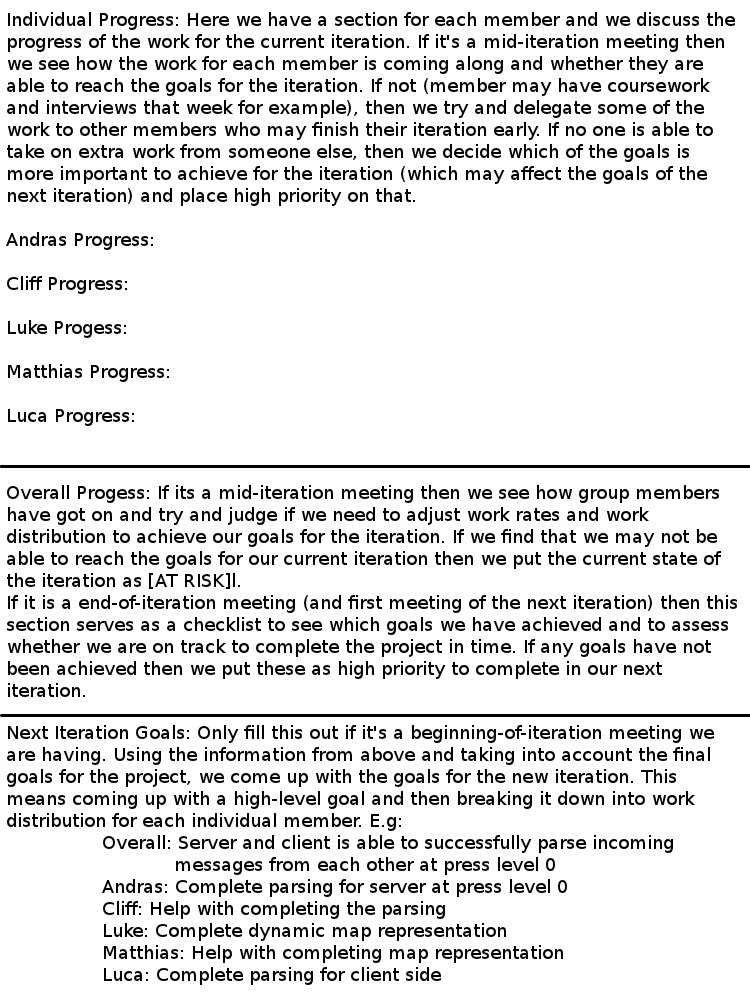
\includegraphics[width=100mm]{logbooktemplate.png}


\subsection{Version control}
The distributed source code control system Git was used for all deliverables -
that is unit tests / documentation, tutorials and presentations. We have made
it strict policy to avoid both conflicting / non-compiling commits. The former
required good coordination between team members about which files should be
edited in what time-window. Any file that is machine-generated should be
ignored by the file tracker to avoid confusion and wasted memory space in
the repository. For simplicity we avoided working on different development
branches. All code was backup-ed in the project directory of DoC at regular
intervals. 

\subsection{Automated build}
The CABAL package management system was used as recommendend by most
Haskell coding standards. The different parts of the project (Server, Client,
AI) were packaged separately to avoid annoying compile dependencies and
allow team members to work separately on different components. In our judgement
a suitable CI server does not exist for Haskell and using one would have been 
overkill.

\subsection{Management / Organisational policies}
We tried to keep it lean here: There is a culture of trust within the group which
can be justified because we have been rigorous about commit / coding rules at the
outset. Sub-optimal design decisions were usually caught in the ``design-check'' sessions 
explained above. For some parts of the codebase exotic techniques like Software
Transactional Memory were used. This proved problematic because team members
usually did not have the time to learn these new concepts, making code review
difficult. In such cases 'research papers' presenting the necessary techniques
were usually sent to each team member involved in the code inspection. We had
to take a pragmatic approach here -- after all team members sometimes have very
different backgrounds in programming paradigms / coding techniques. It is a necessary
side-effect of division of labour that not everybody is an expert in everything.

\subsection{Knowledge transfer within the group}
As previously mentioned, there is a significant amount of knowledge variation
within members of the group. Some of us are skilled with Haskell coding, whilst
some of us are merely acquainted with it. Similarly, GUI design, AI design,
general coding skills and practices all varied. We have remedied this 
somewhat by working in pairs or more, allowing the parts of the knowledge to 
diffuse (in a manner similar to osmosis :) ) between group
members as problems are encountered and solved. Additionally, papers and other
learning tools have been shared (via GitHub and Gmail) to aid the code writing
process. Where  learning-by-application and reading have failed, group members have also been
keen to help each other, spending time drawing UML diagrams and explaining concepts
in detail. The focal points of these discussions have usually been the weekly 
group meetings. Logbook allowed us to document what we have learned and avoid
introducing bad design / bugs more than once. 
\\ 
Last but not least we decided to have a ``glossary'' section in the log-book 
where we explain give names to the most important concepts of our design. For instance
we have defined the AI framework in terms of metaphors from the Neuroscience
domain (Brain etc..). For this to be effective and improve communication every 
team member needed to be aware of the terms.

\section{Contribution of team members}

\section{Self evaluation / reflection}

\subsection{Specification vs. final result}

\subsection{Group collaboration}

\subsection{Technical challenges}

\begin{comment} Possible overlap with change management \end{comment}

\subsection{Learning}



\section{Conclusions}


\section{Future work}

\section{Appendix}

\begin{comment}

User guides, documentation etc, Tutorials, Experiment results (??) 

\end{comment}


\bibliography{report4_refs}

\end{document}
